\part{Celestial $\mathcal{A}$mplitudes \& CCFT}
% 计数器清零,每个part都要引用,除了part1
\setcounter{theorem}{0}
\setcounter{definition}{0}
\setcounter{lemma}{0}
\setcounter{sidenote}{1}
\section{Conformal basis}
QFT中利用费曼图计算散射振幅都是在动量空间下进行的,也就是选取在平面波为基底,这样做最大的好处是可以显现出平移对称性。但是在考虑天球上的散射问题时,很显然我们应当最大化利用共性对称性,所以基底应该选取为类似CFT中初级场的形式,称之为“Conformal Primary Wave Function”,这样$\mathbb{R}^{d+1,1}$上的散射振幅就有希望在这个基底下类似于CFT$_{d}$中的n点关联函数,Clifford Cheung很早就利用这个基底对一些特殊情形进行了研究\cite{Cheung:2016iub}\sn{历史上最早可以追溯到Dirac\cite{436861d5-35f6-36cf-9470-cb587eced490}}。现在顺着文献\cite{Pasterski:2017kqt}的思路来介绍这一组基底。
\subsection{Massive Scalar}
\begin{definition}[Massive Scalar Conformal Primary Wave Function]
自旋为$0$的标量场既没有$\mathbb{R}^{d+1,1}$上的$SO(d+1,1\uparrow$指标,也没有spinning CFT特有的张量指标,或者说处于$SO(d)$的标量表示。对于平面波,我们使用在壳动量来标记基底,现在我们使用$\Delta\in\mathbb{C},\vec{w}$来标记基底。
\begin{itemize}
	\item 在壳:
	\begin{equation}
		\left(\frac{\partial}{\partial X^{\nu}} \frac{\partial}{\partial X_{\nu}}-m^{2}\right) \phi_{\Delta}\left(X^{\mu} ; \vec{w}\right)=0
	\end{equation}
	\item 在共形变换和$SO(d+1,1)$下协变:
	\begin{equation}
		\phi_{\Delta}\left({\Lambda^{\mu}}_{\nu} X^{\nu} ; \vec{w}^{\prime}(\vec{w})\right)=\left|\frac{\partial \vec{w}^{\prime}}{\partial \vec{w}}\right|^{-\Delta / d} \phi_{\Delta}\left(X^{\mu} ; \vec{w}\right)
	\end{equation}
	这里$\vec{w}\to\vec{w}^\prime$是共形变换\footnote{注意,对于$d=2$的情形,对应的是全局共形变换,更类似于准初级场。},${\Lambda^\mu}_\nu$是诱导的Lorentz变换。
\end{itemize}
\end{definition}
后面的讨论使用Embedding形式将$\mathbb{R}^{d}$嵌入到$\mathbb{R}^{d+1,1}$的光锥,再次写下这个嵌入:
\begin{equation}
	q^\mu(\vec{w})=\left(1+|\vec{w}|^2,2\vec{w},1-|\vec{w}|^2\right),\quad q^\mu(\vec{w}^\prime)=\left|\frac{\partial \vec{w}^\prime}{\partial\vec{w}}\right|^{\frac{1}{d}}{\Lambda^\mu}_\nu q^\nu(\vec{w})
\end{equation}
粒子在壳动量$p^2=-m^2$,由于质量是固定的,抽出动量方向得到$\hat p^2=-1$,而这其实就说明$\hat p$位于unit hyperboloid space $\mathbb{H}_{d+1}$上\sn{$\mathbb{H}_{d+1}$表示$d+1$维截面曲率恒为$-1$的超曲面,Killing-Hopf定理保证这样的曲面只有这一种}。可以利用Poincar\'e half-plane对$\mathbb{H}_{d+1}$进行参数化:
\begin{equation}
	ds^2_{\mathbb{H}_{d+1}}=\frac{dy^2+d\vec{z}\cdot d\vec{z}}{y^2},\quad y>0,\vec{z}\in\mathbb{R}^d
\end{equation}
$y=0$对应$\partial\mathbb{H}_{d+1}$。$ds^2_{\mathbb{H}_{d+1}}$天然是$SO(d+1,1)$不变的,也就是在下面的变换下不变:
\begin{itemize}
	\item $\mathbb{R}^d$ translation : $\quad y^{\prime}=y, \quad \vec{z}^{\prime}=\vec{z}+\vec{a}$,\\
	\item $S O(d)$ rotation : $y^{\prime}=y, \quad \vec{z}^{\prime}=M \cdot \vec{z}$,\\
	\item dilation : $\quad y^{\prime}=\lambda y, \quad \vec{z}^{\prime}=\lambda \vec{z}$\\
	\item special conformal transformation : $y^{\prime}=\frac{y}{1+2 \vec{b} \cdot \vec{z}+|\vec{b}|^2\left(y^2+|\vec{z}|^2\right)}, \quad \vec{z}^{\prime}=\frac{\vec{z}+\left(y^2+|\vec{z}|^2\right) \vec{b}}{1+2 \vec{b} \cdot \vec{z}+|\vec{b}|^2\left(y^2+|\vec{z}|^2\right)}$
\end{itemize}
任意在在壳动量$m\hat p$可以参数化为:
\begin{equation}
	\hat{p}(y,\vec{z})=\left(\frac{1+y^2+|\vec{z}|^2}{2y},\frac{\vec{z}}{y},\frac{1-y^2-|\vec{z}|^2}{2y}\right)
\end{equation}
这其实就是在将$\mathbb{H}_{d+1}$嵌入到$\mathbb{R}^{d+1,1}$的未来光锥部分\sn{因为$\hat p^0>0$},比如$\mathbb{R}^{3,1}$的时空图就可以分层为:
\begin{figure}[H]
	\centering 
	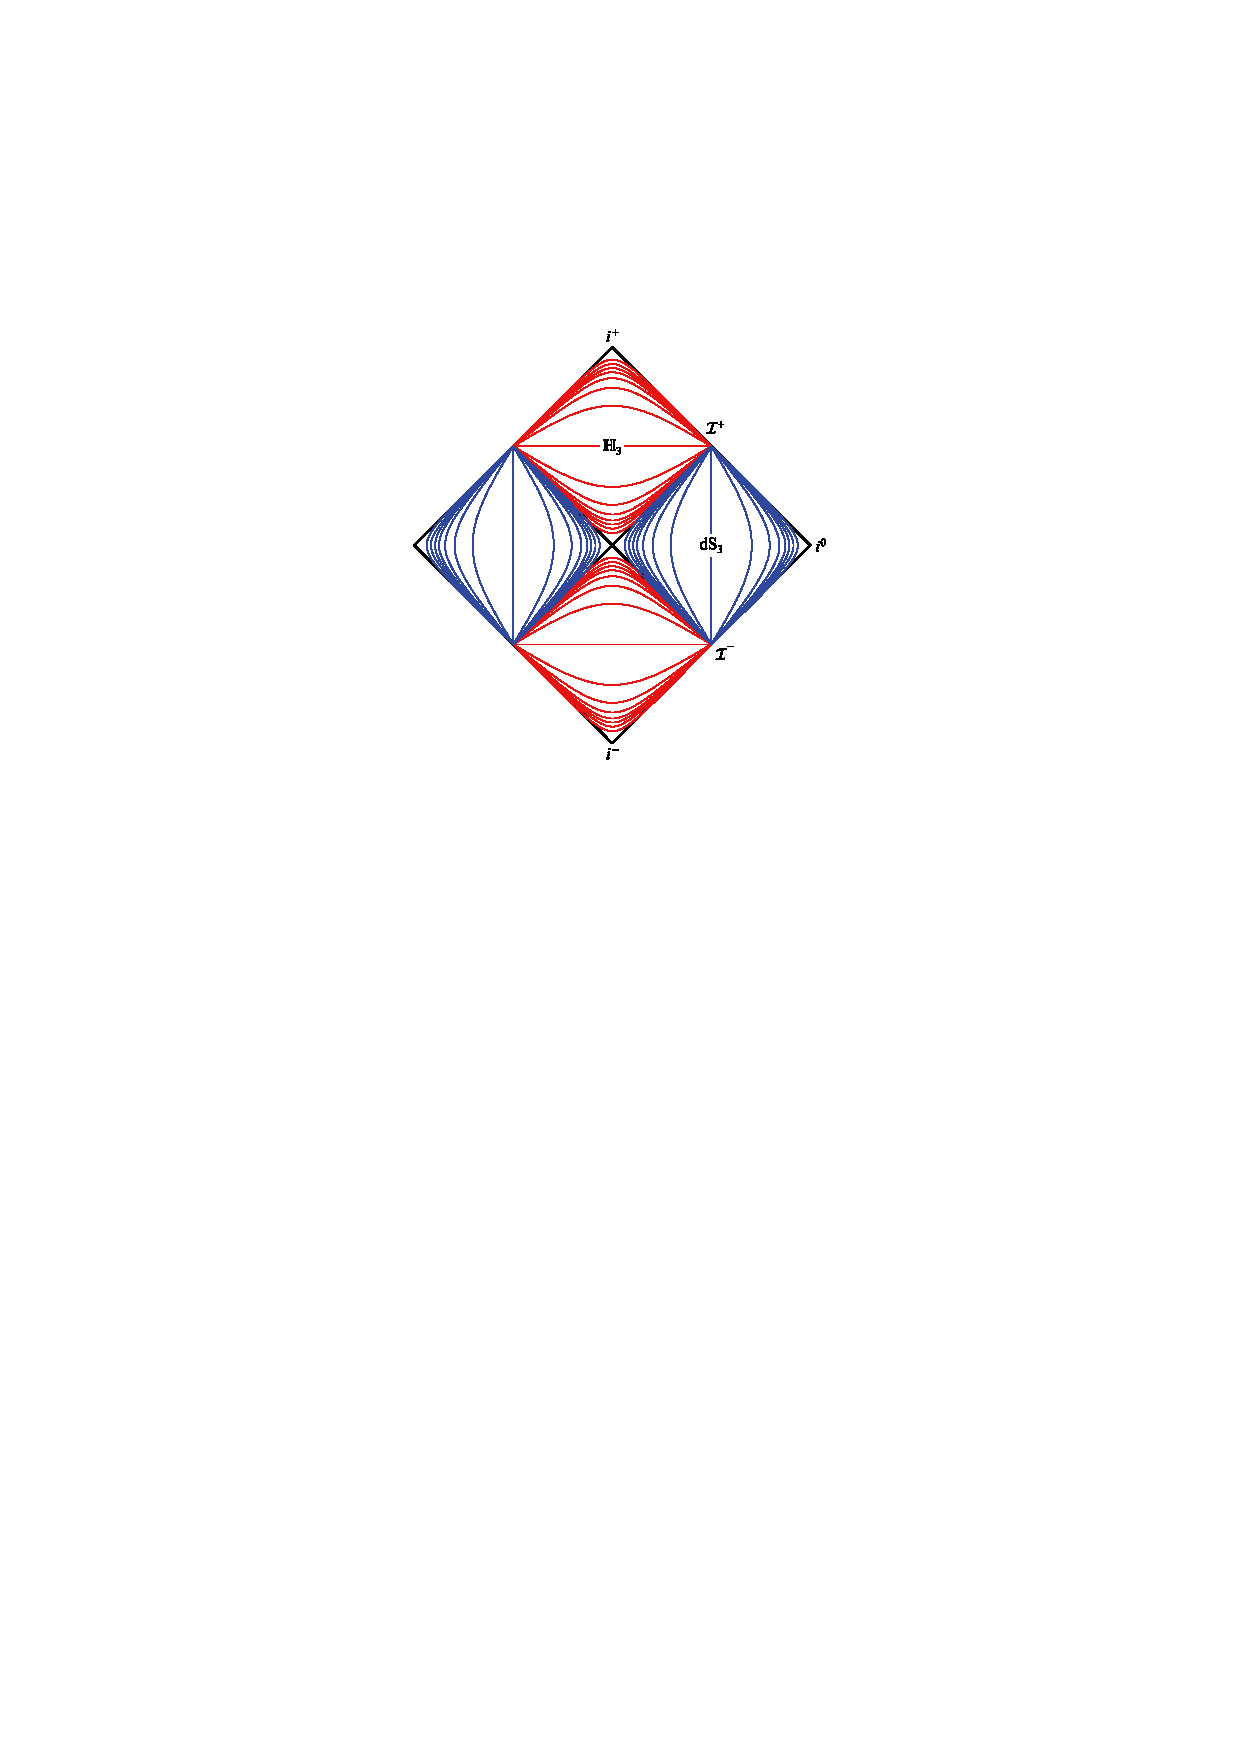
\includegraphics{figs/fig6.pdf}
	\caption{$Mink_4$时空的叶状结构}
\end{figure}
我们只使用unit的那一层。AdS/CFT对偶里面有一个bulk-to-boundary传播子,在前面的参数化下定义为\cite{Witten:1998qj}:
\begin{equation}
	\boxed{
	G_\Delta(\hat{p};\vec{w})=\left(\frac{y}{y^2+|\vec{z}-\vec{w}|^2}\right)^\Delta =G_\Delta(\hat{p};q)=\frac{1}{(-\hat{p}\cdot q)^\Delta}
	}
\end{equation}
这个传播子在共形变换$q\to q^\prime$,以及所诱导的Lorentz变换$\hat p\to\hat p^\prime$下变换性质为:
\begin{equation}
	G_\Delta(\hat{p'};q')=\left|\frac{\partial\vec{w}'}{\partial\vec{w}}\right|^{-\Delta/d}G_\Delta(\hat{p};q)
\end{equation}
最终的基底肯定是用平面波$\exp\left[\pm im\hat{p}\cdot X\right]$线性组合得到的,这里$+$表示out态,$-$表示in态。而且线性组合要对所有在壳动量构成的平面波求和,所以积分是在$\mathbb{H}_{d+1}$上进行的,积分测度是上面的不变测度:
\begin{equation}
	\int_{\mathbb{H}_{d+1}}[d\hat{p}]\equiv\int_0^\infty\frac{dy}{y^{d+1}}\int d^d\vec{z}=\int_{\hat p^2=-1}\frac{d^{d+1}\hat{p}^i}{\hat{p}^0}
\end{equation}
由于KG方程是一个线性方程,所以线性组合之后的结果都是KG方程的解\sn{只要线性组合的系数与$X$无关就好}。由于$G_\Delta$在共形变换下刚好出来我们需要的共形变换因子,而诱导的Lorentz变换本身不贵改变$\hat p \cdot X$和积分测度,所以下面的积分就是满足条件的conformal basis:
\begin{equation}\label{27}
	\boxed{
	\phi_\Delta^\pm(X^\mu;\vec{w})=\int_{\mathbb{H}_{d+1}}[d\hat{p}]G_\Delta(\hat{p};\vec{w})\exp\left[\pm im\hat{p}\cdot X\right]
	}
\end{equation}
注意$\Delta$和$\vec{w}$是用来标记基底的,与$m$无关。但是上面的式子只是形式上的定义,第一不便于计算,第二上式对于$m\in\mathbb{R}_+$是发散的,只有对于$m\in-i{\mathbb{R}_+}$才收敛,所以上式应当看作是先把$m$变成纯虚数积分,然后延拓到实轴。所以考虑直接去找满足条件的KG方程的解,设试探解为:
\begin{equation}
	\phi_\Delta(X^\mu;\vec{w})=\frac{f(X^2)}{(-q\cdot X)^\Delta}
\end{equation}
代入方程得到:
\begin{equation}
	0=4X^2f''(X^2)-2(2\Delta-d-2)f'(X^2)-m^2f(X^2)
\end{equation}
这是虚宗量Bessel方程,考虑$X\to\infty$收敛的解,解正比于第二类修正Bessel函数:
\[f(X^2)\propto\left(\sqrt{-X^2}\right)^{\Delta-\frac{d}{2}}K_{\Delta-\frac{d}{2}}\left(m\sqrt{X^2}\right)\]
前面的比例系数可以从积分表达式\ref{27}积分后最终对比得到:
\begin{equation}
	\phi_\Delta^\pm(X^\mu;\vec{w})=\frac{2^{\frac d2+1}\pi^{\frac d2}}{(im)^{\frac d2}}\frac{(\sqrt{-X^2})^{\Delta-\frac d2}}{(-q(\vec{w})\cdot X\mp i\epsilon)^\Delta}K_{\Delta-\frac d2}(m\sqrt{X^2})
\end{equation}
$\mathcal{A}\equiv\bra{\textbf{out}}\mathcal{S}\ket{\text{in}}$,那么在conformal基底下的散射振幅和原先动量空间散射振幅之间关系为:
\begin{equation}
	\widetilde{\mathcal{A}}(\Delta_i,\vec{w}_i)\equiv\prod_{k=1}^n\int_{\mathbb{H}_{d+1}}[d\hat{p}_k]G_{\Delta_k}(\hat{p}_k;\vec{w}_k)\mathcal{A}(\pm m_i\hat{p}_i^\mu)
\end{equation}
显然其具有CFT中n点关联函数性质:
\begin{equation}
	\widetilde{\mathcal A}(\Delta_{i},\vec{w}_{i}^{\prime}(\vec{w}_{i}))=\prod_{k=1}^{n}\left|\frac{\partial\vec{w}_{k}^{\prime}}{\partial\vec{w}_{k}}\right|^{-\Delta_{k}/d}\widetilde{\mathcal A}(\Delta_{i},\vec{w}_{i})
\end{equation}

前面一直在讲基底,但前面不对$\Delta$进行限制,构造出来的$\{\phi^{\pm}_{\Delta,\vec{w}}\}$极有可能是超完备的。下面我们要干的事情是在构造出来的这些基底里面选某一簇构造正交完备归一基底。

\begin{definition}[shadow transformation]
	对于一个共形维数为$\Delta$的(准)初级场$\mathcal{O}_\Delta(\vec{w})$,其\textbf{shadow}的定义为\cite{Ferrara:1972xe,Ferrara:1972ay,Ferrara:1972uq,Ferrara:1972kab}:
	\begin{equation}
		\begin{aligned}\widetilde{\mathcal{O}}_\Delta(\vec{w})&\equiv\frac{\Gamma(\Delta)}{\pi^{\frac{d}{2}}\Gamma(\Delta-\frac{d}{2})}\int d^d\vec{w}'\frac{1}{|\vec{w}-\vec{w}'|^{2(d-\Delta)}}\mathcal{O}_\Delta(\vec{w}')\end{aligned}
	\end{equation}
	不难发现,场的shadow变成了共形维数为$d-\Delta$的(准)初级场。
\end{definition}
由于$K_\alpha=K_{-\alpha}$,以及下面的恒等式\cite{Simmons-Duffin:2012juh}:
\begin{equation}
	\int d^{d}\vec{z}\frac{1}{|\vec{z}-\vec{w}|^{2(d-\Delta)}}\frac{1}{(-q(\vec{z})\cdot X)^{\Delta}}=\frac{\pi^{\frac{d}{2}}\Gamma(\Delta-\frac{d}{2})}{\Gamma(\Delta)}\frac{(-X^{2})^{\frac{d}{2}-\Delta}}{(-q(\vec{w})\cdot X)^{d-\Delta}}
\end{equation}
得到了一个核心等式:
\begin{equation}\label{eq:27.17}
	\boxed{\widetilde{\phi_\Delta^\pm}(X;\vec{w})=\phi_{d-\Delta}^\pm(X;\vec{w})}
\end{equation}
这实际上直接把空间一分为二,分成某个子空间和它的shadow,我们只用取其中一个构成基就好,因为它的shadow是其线性组合。

在考虑$SO(d+1,1)$的无限维表示\sn{\cite{Sun:2021rrs,Sun:2021thf}这两篇文章比较易读,而且重在比较新,文章\cite{Bissi:2023bhv}的$\S 2.2$是对此内容的一个简短review,更多的阅读材料可以在那里找到。}时会出现所谓\textbf{principal continuous series}的概念:
\begin{equation}
	\boxed{\Delta\in\frac d2+i\mathbb{R}}
\end{equation}
后面构造conformal basis就是用这一series里面的$\Delta$或其子集进行构造,这一点不加证明,后面只是去说明这样确实能得到正确的基底。

首先注意到关于$G_\Delta$的几个正交完备性关系\cite{Costa:2014kfa}:
\begin{equation}
	\int_{-\infty}^{\infty}d\nu\mu(\nu)\int d^{d}\vec{w}G_{\frac{d}{2}+i\nu}(\hat{p}_{1};\vec{w})G_{\frac{d}{2}-i\nu}(\hat{p}_{2};\vec{w})=\delta^{(d+1)}(\hat{p}_{1},\hat{p}_{2})
\end{equation}
这里$\delta$函数是定义在$\mathbb{H}_{d+1}$上也就是$SO(d+1,1)$不变的,积分测度$\mu(\nu)$:
\begin{equation}
	\mu(\nu)=\frac{\Gamma(\frac d2+i\nu)\Gamma(\frac d2-i\nu)}{4\pi^{d+1}\Gamma(i\nu)\Gamma(-i\nu)}
\end{equation}
还有一个
\begin{equation}
	\begin{gathered}
		\int_{H_{d+1}}[d\hat{p}]G_{\frac d2+i\nu}(\hat{p};\vec{w}_{1})G_{\frac d2+i\bar{\nu}}(\hat{p};\vec{w}_{2})= \\
		2\pi^{d+1}\frac{\Gamma(i\nu)\Gamma(-i\nu)}{\Gamma(\frac d2+i\nu)\Gamma(\frac d2-i\nu)}\delta(\nu+\bar{\nu})\delta^{(d)}(\vec{w}_{1}-\vec{w}_{2})+2\pi^{\frac d2+1}\frac{\Gamma(i\nu)}{\Gamma(\frac d2+i\nu)}\delta(\nu-\bar{\nu})\frac{1}{|\vec{w}_{1}-\vec{w}_{2}|^{2(\frac d2+i\nu)}}.
	\end{gathered}
\end{equation}
利用这些关系可以得到\ref{27}的逆变换:
\begin{equation}
	\boxed{e^{\pm im\hat{p}\cdot X}=2\int_0^\infty d\nu\mu(\nu)\int d^d\vec{w}G_{\frac d2-i\nu}(\hat{p};\vec{w})\phi_{\frac d2+i\nu}^\pm(X^\mu;\vec{w})}
\end{equation}
由于平面波基底完备,逆变换的存在性立刻就说明了利用principal continuous series构造出来的$\{\phi^{\pm}_{\Delta,\vec{w}}\}$也完备,而且注意到我们这里利用\ref{eq:27.17}将$\nu$限制在了$\mathbb{R}_+$上,所以:
\begin{equation}\label{eq:27.23}
	\boxed{\Delta\in\frac d2+i\mathbb{R}_{\geq 0}}
\end{equation}
这佐证了前面提到的只需要在空间和其shadow里面取一个就好了。正交性依赖于内积的定义,这里自然的定义KG内积:
\begin{equation}
	(\Phi_1,\Phi_2)=-i\int_\Sigma d^{d+1}X^i\left[\Phi_1(X)\partial_{X^0}\Phi_2^*(X)-\partial_{X^0}\Phi_1(X)\Phi_2^*(X)\right]
\end{equation}
这个定义是Poincar\'e不变的,是与Cauchy面选取无关的。计算得到:
\begin{equation}
	\begin{aligned}
		\left(\phi_{\frac{d}{2}+i\nu_{1}}^{\pm}(X^{\mu};\vec{w_{1}})\right.,&\left.\phi_{\frac{d}{2}+i\nu_{2}}^{\pm}(X^{\mu};\vec{w_{2}})\right) \\
		=&\pm\frac{2^{d+3}\pi^{2d+2}}{m^{d}}\frac{\Gamma(i\nu_{1})\Gamma(-i\nu_{1})}{\Gamma(\frac{d}{2}+i\nu_{1})\Gamma(\frac{d}{2}-i\nu_{1})}\delta(\nu_{1}-\nu_{2})\delta^{(d)}(\vec{w}_{1}-\vec{w}_{2}) \\
		&\pm\cancelto{0}{\frac{2^{d+3}\pi^{\frac{3d}{2}+2}}{m^{d}}\frac{\Gamma(i\nu_{1})}{\Gamma(\frac{d}{2}+i\nu_{1})}\delta(\nu_{1}+\nu_{2})\frac{1}{|\vec{w}_{1}-\vec{w}_{2}|^{2(\frac{d}{2}+i\nu_{1})}}}
	\end{aligned}
\end{equation}
第二项为$0$是因为\ref{eq:27.23}。总结一下,我们得到了$\ket{\text{in}}$和$\ket{\text{out}}$态的基底为:
\begin{equation}
	\boxed{\mathcal{B}^{\pm}=\left\{\begin{array}{c|c}\phi_{\frac{d}{2}+i\nu}^{\pm}(X;\vec{w})&\nu\geq0,\vec{w}\in\mathbb{R}^d\end{array}\right\}}
\end{equation}
它的shadow同样是一组基底:
\begin{equation}
	\boxed{\widetilde{\mathcal{B}}^\pm=\left\{\begin{array}{c|c}\phi_{\frac{d}{2}+i\nu}^\pm(X;\vec{w})&\nu\le0,\vec{w}\in\mathbb{R}^d\end{array}\right\}}
\end{equation}
\subsection{Massless Scalar}
无质量情况看作是有质量情况的极限,作换元$\omega\equiv\frac{m}{2y}$,积分核有如下渐近行为:
\begin{equation}
	G_{\Delta}(y,\vec{z};\vec{w})\xrightarrow{m\to0}\pi^{\frac{d}{2}}\frac{\Gamma(\Delta-\frac{d}{2})}{\Gamma(\Delta)}y^{d-\Delta}\delta^{(d)}(\vec{z}-\vec{w})+\frac{y^{\Delta}}{|\vec{z}-\vec{w}|^{2\Delta}}+\cdots 
\end{equation}
计算得到:
\begin{equation}
	\begin{aligned}\phi_{\frac{d}{2}+i\nu}^{\pm}(X;\vec{w})\xrightarrow{m\to0}&\left(\frac{m}{2}\right)^{-\frac{d}{2}-i\nu}\frac{\pi^{\frac{d}{2}}\Gamma(i\nu)}{\Gamma(\frac{d}{2}+i\nu)}\int_{0}^{\infty}d\omega\omega^{\frac{d}{2}+i\nu-1}e^{\pm i\omega q(\vec{w})\cdot X}\\+&\left(\frac{m}{2}\right)^{-\frac{d}{2}+i\nu}\int d^{d}\vec{z}\frac{1}{|\vec{z}-\vec{w}|^{2(\frac{d}{2}+i\nu)}}\int_{0}^{\infty}d\omega\omega^{\frac{d}{2}-i\nu-1}e^{\pm i\omega q(\vec{z})\cdot X}\end{aligned}
\end{equation}
上面的极限不是well-define的,因为$m^{\pm i\nu}$,但这是个相位,不妨先丢掉,而第二项是第一项的shadow,所以猜测最终应该是下面的形式:
\begin{equation}
	\boxed{\varphi_\Delta^\pm(X^\mu;\vec w)\equiv\int_0^\infty d\omega\omega^{\Delta-1}e^{\pm i\omega q\cdot X-\epsilon\omega}=\frac{(\mp i)^\Delta\Gamma(\Delta)}{(-q(\vec w)\cdot X\mp i\epsilon)^\Delta}}
\end{equation}
其中$\Delta\in\mathbb{C}$,需要重新去找寻。这个式子的形式就是所谓\textbf{Mellin变换}\sn{数学上Mellin变换定义为:\[\widetilde{f}(\Delta)=\int_0^\infty d\omega\omega^{\Delta-1}f(\omega)\]其逆变换为:\[f(\omega)=\frac1{2\pi i}\int_{c-i\infty}^{c+i\infty}d\Delta\omega^{-\Delta}\widetilde{f}(\Delta),c\in\mathbb{R}\]},可以解释成对未来光锥上的某一条射线积分,也就是把所有同“方向”,不同“能量”的平面波组合。注意这个式子有个非常明显的特征,在除去一个归一化因子的意义下,上式结果与$G_\Delta$将$q$替换为$X$得到的结果完全一致。上面变换的逆变换为:
\begin{equation}
	e^{\pm i\omega q\cdot X-\epsilon\omega}=\int_{-\infty}^{\infty}\frac{d\nu}{2\pi}\omega^{-\Delta}\frac{(\mp i)^{\Delta}\Gamma(
		\Delta)}{(-q\cdot X\mp i\epsilon)^{\Delta}},\quad\omega>0,\Re(\Delta)>0
\end{equation}
这说明了$\Re(\Delta)>0$就能保证完备性,而且这组基底张成的空间中很重要的一点是不含零动量的平面波解\sn{这一点是必须的,因为他是KG方程没有物理意义的解,要抛弃掉}。如果选取$\Re(\Delta)=\frac{d}{2}$,$\Im(\Delta)\in\mathbb{R}$,则:
\begin{equation}
	\begin{pmatrix}\varphi_{\frac{d}{2}+i\nu_{1}}^{\pm}(X^{\mu};\vec{w}_{1}),\varphi_{\frac{d}{2}+i\nu_{2}}^{\pm}(X^{\mu};\vec{w}_{2})\end{pmatrix}=\pm8\pi^{d+2}\delta(\nu_{1}-\nu_{2})\delta^{(d)}(\vec{w}_{1}-\vec{w}_{2})
\end{equation}
这个时候注意shadow:
\begin{equation}
	\begin{aligned}
		\widetilde{\varphi_{\frac{d}{2}+i\nu}^{\pm}}(X^{\mu};\vec{w})& =\frac{\Gamma(\frac{d}{2}+i\nu)}{\pi^{\frac{d}{2}}\Gamma(i\nu)}\int d^{d}\vec{z}\frac{1}{|\vec{z}-\vec{w}|^{2(\frac{d}{2}-i\nu)}}\varphi_{\frac{d}{2}+i\nu}^{\pm}(X^{\mu};\vec{z})  \\
		&=(\mp i)^{\frac d2+i\nu}\Gamma(\frac d2+i\nu)\frac{(-X^2)^{-i\nu}}{(-q(\vec{w})\cdot X\mp i\epsilon)^{\frac d2-i\nu}}\\
		\left(\varphi_{\frac{d}{2}+i\nu_1}^{\pm}(X^{\mu};\vec{w_1}),\right.&\left.\widetilde{\varphi_{\frac{d}{2}+i\nu_2}^{\pm}}(X^{\mu};\vec{w_2})\right)=\pm8\pi^{\frac{d}{2}+2}\frac{\Gamma(\frac{d}{2}-i\nu_1)}{\Gamma(-i\nu_1)}\delta(\nu_1-\nu_2)\frac{1}{|\vec{w_1}-\vec{w_2}|^{2(\frac{d}{2}+i\nu_1)}}
	\end{aligned}
\end{equation}
其shadow当然也是一组基底,但并不是$\nu\to-\nu$这么简单了,这导致$\nu$的取值范围也拓宽到了所有实数。总结一下,我们得到了Massless scalar的conformal basis:
\begin{equation}
	\boxed{\mathcal{B}_{m=0}^{\pm}=\left\{\begin{array}{c|c}\varphi_{\frac{d}{2}+i\nu}^{\pm}(X^{\mu};\vec{w})&\nu\in\mathbb{R},\vec{w}\in\mathbb{R}^{d}\end{array}\right\}}
\end{equation}
其shadow也可以作为一组基:
\begin{equation}
	\boxed{\widetilde{\mathcal{B}}_{m=0}^{\pm}=\left\{\begin{array}{c|c}\widetilde{\varphi_{\frac{d}{2}+i\nu}^{\pm}}(X^{\mu};\vec{w})&\nu\in\mathbb{R},\vec{w}\in\mathbb{R}^{d}\end{array}\right\}}
\end{equation}
\subsection{photon \& Graviton}
这两个除了自旋不为0,还有一个比较麻烦的点是需要取定规范。由于自旋不为0,所以基底除了在壳动量、初末态的$\pm$,以及极化矢量带来的$SO(1,d+1)$矢量指标,还需要一个指标用来标记自旋,这里考虑的是无质量玻色子,所以这个指标标记的是粒子的螺旋度,体现为CFT$_d$上的一个$\mathbb{R}^d$张量指标,$a=1,2,\ldots,d$。令在壳动量$k=\omega q$,在Loren规范下可以把平面波基底写为下面的形式:\sn{\[\partial_aq^\mu\equiv\frac{\partial}{\partial w^a}q^\mu(\vec{w})=2(w^a,\delta^{ba},-w^a)\]}:
\begin{equation}
	\partial_aq_\mu e^{\pm i\omega q\cdot X}
\end{equation}
注意Lorenz规范只能将前面的极化矢量确定到一个正比于$k$的项,选取这样的形式相当于完全取定了规范。不难验证$d=2$时,上面的选取就对应\ref{eq:24.7}的选取。
\begin{definition}[Spin\mbox{-}1 Massless Boson, $d\geq 1$]
	~
	\begin{itemize}
		\item 在壳:\footnote{满足的是Proca方程}
		\begin{equation}
			\left(\frac{\partial}{\partial X^\sigma}\frac{\partial}{\partial X_\sigma}\delta_\nu^\mu-\frac{\partial}{\partial X^\nu}\frac{\partial}{\partial X_\mu}\right)A_{\mu a}^{\Delta\pm}(X^\rho;\vec{w})=0
		\end{equation}
		\item 协变:
		\begin{equation}
			A_{\mu a}^{\Delta\pm}\left(\Lambda^{\rho}{}_{\nu}X^{\nu};\vec{w}'(\vec{w})\right)=\frac{\partial w^{b}}{\partial{w'^{a}}}\left|\frac{\partial\vec{w}'}{\partial\vec{w}}\right|^{-(\Delta-1)/d}\Lambda_{\mu}{}^{\sigma}A_{\sigma b}^{\Delta\pm}(X^{\rho};\vec{w})
		\end{equation}
	\end{itemize}
\end{definition}
$\mathbb{H}_{d+1}$上面的 Spin\mbox{-}1 bulk-to boundary 传播子为$G^\Delta_{\mu;q}$\sn{后面只要是$a,b,c$指标就是$\mathbb{R}^d$上的,在只要是$\mu,\nu,\sigma$指标就是$\mathbb{R}^{1,d+1}$上的},计算上更常用的是其 \textbf{uplift} $G^\Delta_{\mu;\nu}$,定义为:\sn{其实就是拉回映射}
\begin{equation}
	G^\Delta_{\mu;q}=\frac{\partial q^\nu}{\partial w^a}G_{\mu;\nu}^\Delta(\hat{p};q)
\end{equation}
\begin{equation}
	G_{\mu;\nu}^{\Delta}(\hat{p};q)=\frac{(-q\cdot\hat{p})\eta_{\mu\nu}+q_{\mu}\hat{p}_{\nu}}{(-q\cdot\hat{p})^{\Delta+1}}
\end{equation}
uplift之后,$G^\Delta_{\mu;\nu}$就是一个标量CFT$_d$,而且是$\mathbb{R}^{1,d+1}$上的2\mbox{-}tensor:
\begin{equation}
	G_{\mu;\nu}^{\Delta}(\Lambda\hat{p};\Lambda q)=\left|\frac{\partial\vec{w}'}{\partial\vec{w}}\right|^{-\Delta/d}\Lambda^{\rho}{}_{\mu}\Lambda^{\sigma}{}_{\nu}G^{\Delta}{}_{\rho;\sigma}(\hat{p};q)
\end{equation}
而且关于两个自变量还满足横向条件:
\begin{equation}\label{eq:t}
	\hat{p}^{\mu}G_{\mu;\nu}^{\Delta}(\hat{p};q)=0,\quad q^{\nu}G_{\mu;\nu}^{\Delta}(\hat{p};q)=0
\end{equation}
根据前面的标量场经验,不难猜测$A$的形式就是$G$把$q$换成$X$:
\begin{equation}
	\boxed{
		\begin{aligned}
			A_{\mu a}^{\Delta,\pm}(X^{\mu};\vec{w})& {=\frac{\partial_{a}q_{\mu}}{(-q\cdot X\mp i\epsilon)^{\Delta}}+\frac{\partial_{a}q\cdot X}{(-q\cdot X\mp i\epsilon)^{\Delta+1}}q_{\mu}} \\
			&=-\frac{1}{(-q\cdot X\mp i\epsilon)^{\Delta-1}}\frac{\partial}{\partial X^{\mu}}\frac{\partial}{\partial w^{a}}\log(-q\cdot X\mp i\epsilon)
		\end{aligned}
	}
\end{equation}
证明略。下面计算其shadow。
\begin{definition}[shadow for spinning fields]
	对于自旋为$J$的场,其会导致带有$J$个$\mathbb{R}^d$上的指标$a_1,\ldots,a_J$,而且这些指标是无迹且全对称的,或者说$\mathcal{O}^\Delta_{a_1\cdot\cdot\cdot a_J}(\vec{w})$是$SO(d)$的无迹对称张量表示,即Spin\mbox{-}J表示。计算其shadow最简单的方式是使用其uplift计算,然后再投影回来,uplift与其自身的关系为:
	\begin{equation}
		\mathcal{O}^\Delta_{a_1\cdots a_J}(\vec{w})=\frac{\partial q^{\mu_1}}{\partial w^{a_1}}\cdots\frac{\partial q^{\mu_J}}{\partial w^{a_J}}\mathcal{O}^\Delta_{\mu_1\cdots\mu_J}(\vec{w})
	\end{equation}
	uplift与其自变量之间存在类似\ref{eq:t}的横向关系。
	\begin{equation}
		\boxed{
		\widetilde{\mathcal{O}^\Delta}_{\mu_1\cdots\mu_J}(\vec{w})=\frac{\Gamma(\Delta+J)}{\pi^{\frac d2}(\Delta-1)_J\Gamma(\Delta-\frac d2)}\int d^d\vec{w}^{\prime}\frac{\prod_{n=1}^J\left[\delta_{\mu_n}^{\nu_n}(-\frac12q\cdot q^{\prime})+\frac12q_{\mu_n}^{\prime}q^{\nu_n}\right]}{(-\frac12q\cdot q^{\prime})^{d-\Delta+J}}\mathcal{O}^\Delta_{\nu_1\cdots\nu_J}(\vec{w}^{\prime})}
	\end{equation}
	这里$(a)_{J}\equiv\Gamma(a+J)/\Gamma(a)$,称为Pochhammer符号,而且不难发现上面的定义对于某些$\Delta$不是well-define的,所以需要解析延拓到全部复平面。
\end{definition}
利用上面定义计算得到:
\begin{equation}
	\boxed{
	\widetilde{A_{\mu a}^{\Delta,\pm}}(X^\mu;\vec{w})=(-X^2)^{\frac{d}{2}-\Delta}A_{\mu a}^{d-\Delta,\pm}(X^\mu;\vec{w})
	}
\end{equation}
和无质量标量场一样,不是正比于$A_{\mu a}^{d-\Delta,\pm}$。现在还没有讨论我们的计算是在哪个规范下进行的,但其实前面对$A_{\mu a}^{\Delta,\pm}$那些在壳协变的要求就已经为我们完全取定了规范,是Lorenz和radial规范同时加上去:\sn{这两个规范是可以同时取的,见\cite{PhysRevD.76.084013}}
\begin{equation}
	X^{\mu}A_{\mu a}^{\Delta,\pm}(X^{\mu};\vec{w})=0,\quad\partial^{\mu}A_{\mu a}^{\Delta,\pm}(X^{\mu};\vec{w})=0.
\end{equation}
下表总结了$A_{\mu a}^{\Delta,\pm}$及其 shadow 为 pure gauge\sn{pure gauge就是说可以从$A=0$通过规范变换变过来,所以场强张量为0,$A$可以写为$\frac{i}{g}U\partial_\mu U^\dagger$的形式}的条件:
\begin{center}
	\begin{tabular}[H]{|c|c|c|}
		\hline & $d=2$ & $d \neq 2$ \\
		\hline$A_{\mu a}^{\Delta, \pm}$ & & $\Delta=1$ \\
		& $\Delta=1$ & \\
		$\widetilde{A_{\mu a}^{d-\Delta, \pm}}$& & $\times$ \\
		\hline
	\end{tabular}
\end{center}
回顾一些前面给的平面波基底是在Lorenz规范下给的,不一定满足radial规范,所以$A$不能写成平面波基底的积分变换形式,但是:
\begin{equation}
	\boxed{
	\varphi_{\mu a}^{\Delta,\pm}(X^{\mu};\vec{w})=\int_0^\infty d\omega\omega^{\Delta-1}\left(\partial_aq_\mu e^{\pm i\omega q\cdot X-\epsilon\omega}\right)=(\mp i)^\Delta\Gamma(\Delta)\frac{\partial_aq_\mu}{(-q\cdot X\mp i\epsilon)^\Delta}
	}
\end{equation}
和$A_{\mu a}^{\Delta,\pm}$之间只差一个规范变换\sn{$\frac{\partial}{\partial X^\mu}\left(\frac{\partial_aq\cdot X}{(-q\cdot X\mp i\epsilon)^\Delta}\right)$},那么在计算散射振幅这种与规范选取无关的物理量的时候,用两组基底都能得到同样的结果,但是注意用$\varphi_{\mu a}^{\Delta,\pm}$做基底的时候就没有协变的条件了,但是好处在两基底振幅之间是Mellin变换的形式。在下面的内积定义下:
\begin{equation}
	(A_{\mu},A'_{\mu'})=-i\int _\Sigma d^{d+1}X^i\left[A^{\rho}F'^*_{0\rho}-A'^{\rho*}F_{0\rho}\right]
\end{equation}
当选取$\boxed{\Delta\in\frac{d}{2}+\mathrm{i}\mathbb{R}}$时构成完备基底,其shadow亦然。

这组基底虽说是photon的,但实际上非阿贝尔情形也完全适用,因为每个色指标的场满足相同的方程,相同的协变条件,所以上面的推导完全不变,这是很容易接受的,因为平面波基底对于photon和gluon都是一样通用的。

现在来看引力子的情况,首先在Lorenz\sn{$\partial^{\mu}h_{\mu\nu}-\frac12\partial_{\nu}h^{\rho}{}_{\rho}=0,$}、无迹规范下平面波基底可以写为:
\begin{equation}
	g_{\mu\nu;a_1a_2}^{\pm}(X;\omega,q)=P_{a_1a_2}^{b_1b_2}\partial_{b_1}q_\mu\partial_{b_2}q_\nu e^{\pm i\omega q\cdot X}
\end{equation}
这里:
\begin{equation}
	P_{a_1a_2}^{b_1b_2}\equiv\delta_{(a_1}^{b_1}\delta_{a_2)}^{b_2}-\frac{1}{d}\delta_{a_1a_2}\delta^{b_1b_2}
\end{equation}
\begin{definition}[Graviton, $d\geq 2$]
	~
	\begin{itemize}
		\item 指标约束:
		\begin{equation}
			\begin{array}{l}h_{\mu_1\mu_2;a_1a_2}^{\Delta,\pm}=h_{\mu_2\mu_1;a_1a_2}^{\Delta,\pm},\\h_{\mu_1\mu_2;a_1a_2}^{\Delta,\pm}=h_{\mu_1\mu_2;a_2a_1}^{\Delta,\pm},\quad\delta^{a_1a_2}h_{\mu_1\mu_2;a_1a_2}^{\Delta,\pm}=0\end{array}
		\end{equation}
		第一个约束是几何上要求度规对称,第二个是要求$\mathbb{R}^d$指标无迹且对称。
		\item 在壳:\footnote{满足的是Linearized Einstein方程}
		\begin{equation}
			\partial_\sigma\partial_\nu {h^\sigma}_{\mu;a_1a_2}+\partial_\sigma\partial_\mu {h^\sigma}_{\nu;a_1a_2}-\partial_\mu\partial_\nu {h^\sigma}_{\sigma;a_1a_2}-\partial^\rho\partial_\rho h_{\mu\nu;a_1a_2}=0
		\end{equation}
		\item 协变:
		\begin{equation}
			h_{\mu_1\mu_2;a_1a_2}^{\Delta,\pm}\left(\Lambda_{\nu}^{\rho}X^{\nu};\vec{w}'(\vec{w})\right)=\frac{\partial w^{b_1}}{\partial w'^{a_1}}\frac{\partial w^{b_2}}{\partial w'^{a_2}}\left|\frac{\partial\vec{w'}}{\partial\vec{w}}\right|^{-(\Delta-2)/d}\Lambda_{\mu_1}^{\sigma_1}\Lambda_{\mu_2}^{\sigma_2}h_{\sigma_1\sigma_2;b_1b_2}^{\Delta,\pm}(X^\rho;\vec{w})
		\end{equation}
	\end{itemize}
\end{definition}
利用$\mathbb{H}_{d+1}$上面的 Spin\mbox{-}2 bulk-to boundary 传播子:
\begin{equation}\label{eq:27.55}
	\boxed{
		\begin{aligned}
			h_{\mu_1\mu_2;a_1a_2}^{\Delta,\pm}(X;\vec{w})&=P_{a_1a_2}^{b_1b_2}\frac{\left[(-q\cdot X)\partial_{b_1}q_{\mu_1}+(\partial_{b_1}q\cdot X)q_{\mu_1}\right]\left[(-q\cdot X)\partial_{b_2}q_{\mu_2}+(\partial_{b_2}q\cdot X)q_{\mu_2}\right]}{(-q\cdot X)^{\Delta+2}}\\
			&=P_{a_{1}a_{2}}^{b_{1}b_{2}}\frac{1}{(-q\cdot X\mp i\epsilon)^{\Delta-2}}\partial_{b_{1}}\partial_{\mu_{1}}\log(-q\cdot X\mp i\epsilon)\partial_{b_{2}}\partial_{\mu_{2}}\log(-q\cdot X\mp i\epsilon)
		\end{aligned}
		}
\end{equation}
其shadow:
\begin{equation}
	\widetilde {h_{\mu_1\mu_2;a_1a_2}^{\Delta,\pm}}(X;\vec{w})=(-X^2)^{\frac{d}{2}-\Delta}h_{\mu_1\mu_2;a_1a_2}^{d-\Delta,\pm}(X;\vec{w})
\end{equation}
前面实际上选取了规范:
\begin{equation}
	\eta^{\mu_1\mu_2}h_{\mu_1\mu_2;a_1a_2}^{\Delta,\pm}=0,\quad\partial^{\mu}h_{\mu\mu_2;a_1a_2}^{\Delta,\pm}=0,\quad X^{\mu}h_{\mu\mu_2;a_1a_2}^{\Delta,\pm}=0
\end{equation}
有Pure gauge条件:\sn{可以写为$\partial_{(\mu}\xi_{\nu)}$的形式}
\begin{center}
	\begin{tabular}[H]{|c|cc|c|}
		\hline & \multicolumn{2}{c|}{$d=2$} & $d \geq 2$ \\
		\hline$h_{\mu_1\mu_2;a_1a_2}^{\Delta,\pm}$ & &$\Delta=0$& $\Delta=0,1$ \\
		& $\Delta=1$ & & \\
		$\widetilde{h_{\mu_1\mu_2;a_1a_2}^{d-\Delta,\pm}}$& &$\Delta=2$ & $\times$ \\
		\hline
	\end{tabular}
\end{center}
同样,前面的平面波基底不满足radial规范,但利用Mellin变换后得到的:
\begin{equation}
	\boxed{
	\begin{aligned}
		\varphi_{\mu_1\mu_2;a_1a_2}^{\Delta,\pm}(X^\mu;\vec{w})&=\int_0^\infty d\omega\omega^{\Delta-1}g_{\mu_1\mu_2;a_1a_2}^{\Delta,\pm}(X^\mu;\omega,q^\mu)\\&=(\mp i)^\Delta\Gamma(\Delta)P_{a_1a_2}^{b_1b_2}\frac{\partial_{b_1}q_{\mu_1}\partial_{b_2}q_{\mu_2}}{(-q\cdot X\mp i\epsilon)^\Delta}
	\end{aligned}
}
\end{equation}
与\ref{eq:27.55}只差一个规范变换\begin{margintable}\footnotesize 
	\begin{tabularx}{\marginparwidth}{|X}
		Because:
		\[\frac{\partial_bq_{(\mu_1}q_{\mu_2)}}{(-q\cdot X)^\Delta}=\frac{\partial_{(\mu_1}}{\Delta-1}\left(\frac{\partial_bq_{\mu_2)}}{(-q\cdot X)^{\Delta-1}}\right)\]
		\[\frac{q_{\mu_1}q_{\mu_2}}{(-q\cdot X)^\Delta}=\frac{\partial_{(\mu_1}}{\Delta-1}\left(\frac{q_{\mu_2)}}{(-q\cdot X)^{\Delta-1}}\right)\]
	\end{tabularx}
\end{margintable}。在下面的内积意义下:
\begin{equation}
	\begin{aligned}
		(h_{\mu\nu},h_{\mu^{\prime}\nu^{\prime}}^{\prime})& =-i\int d^{d+1}X^{i}\Big[h^{\mu\nu}\partial_{0}{h^{\prime}}_{\mu\nu}^{*}-2h^{\mu\nu}\partial_{\mu}{h^{\prime}}_{0\nu}^{*}+h\partial^{\mu}{h^{\prime}}_{0\mu}^{*}-h\partial_{0}{h^{\prime}}^{*}+h_{0\mu}{\partial^{\mu}{h^{\prime}}^{*}}  \\
		&-(h\leftrightarrow{h^{\prime}}^{*})\Big]
	\end{aligned}
\end{equation}
$\boxed{\Delta\in\frac{d}{2}+\mathrm{i}\mathbb{R}}$时构成完备基底,其shadow亦然。
\begin{remark}
	$SO(1,d+1)$群的无限维不可约幺正表示由共形维数$\Delta\in\mathbb{C}$和$SO(d)$的表示去标记(或者说取决于对应的$SO(d)$是哪个自旋表示)。前面找的基底就是在找表示,$\Delta$和$J$之间是有约束的,具体来说有下面几个Series:
	\begin{itemize}
		\item Principal Series $\mathcal{P}$: $\forall J\in\mathbb{N},\quad \Delta\in\frac{d}{2}+\mathrm{i}\mathbb{R}$
		\item Complementary Series $\mathcal{C}$: $\Delta=\frac{d}{2}+c$,其中$J=0$时$0<|c|\leq\frac{d}{2}$,$J\geq 1$时$0<|c|\leq\frac{d}{2}-1$
		\item Discrete Series $\mathcal{D}$: 对于奇数维数$d$,任意$J$,$\Delta$可取半整数或者整数
	\end{itemize}
	表示$[\Delta,J]$的shadow就是表示$[d-\Delta,J]$,这两个表示是等价表示。
\end{remark}
\newpage
\subsection{Restrict to Mink$_{4}$}
根据前面的一系列一般性讨论,回到Mink$_{4}$情况很简单,这里只是用文献中比较常用的记号重新写一遍。\sn{\cite{Donnay:2020guq}$\S 2$基本上是很好的总结}

标量场:
\begin{equation}
	\phi_{\Delta,m}\left(\Lambda^{\mu}{}_{\nu}X^{\nu};\frac{aw+b}{cw+d},\frac{\bar{a}\bar{w}+\bar{b}}{\bar{c}\bar{w}+\bar{d}}\right)=|cw+d|^{2\Delta}\phi_{\Delta,m}(X^{\mu};w,\bar{w})
\end{equation}

无质量规范玻色子:
\begin{equation}
	A_{\mu;a}^{\Delta,\pm}\left({\Lambda^{\rho}}_{\nu}X^{\nu};\frac{aw+b}{cw+d},\frac{\bar{a}\bar{w}+\bar{b}}{\bar{c}\bar{w}+\bar{d}}\right)=(cw+d)^{2h}(\bar{c}\bar{w}+\bar{d})^{2\bar{h}}{\Lambda_{\mu}}^{\sigma}A_{\sigma;a}^{\Delta,\pm}(X^{\rho};w,\bar{w})
\end{equation}
无质量规范玻色子只有两种螺旋度选取,对应这里$a=w,\bar w$,分别有$J=+1,-1$。

引力子:
\begin{equation}
	h_{\mu\nu;a}^{\Delta,\pm}\left(\Lambda^{\mu}{}_{\nu}X^{\nu};\frac{aw+b}{cw+d},\frac{\bar{a}\bar{w}+\bar{b}}{\bar{c}\bar{w}+\bar{d}}\right)=(cw+d)^{\Delta+J}(\bar{c}\bar{w}+\bar{d})^{\Delta-J}{\Lambda_{\mu}}^{\rho}{\Lambda_{\nu}}^{\sigma}h_{\rho\sigma,a}^{\Delta,\pm}(X^{\mu};w,\bar{w})
\end{equation}
同样的引力子也只有两种螺旋度选取,对应$a=ww,\bar w\bar w$,分别对应$J=+2,-2$。
不难看出这些情况共形权$(h,\bar h)=\frac12(\Delta+J,\Delta-J)$,$h-\bar h$确实就对应自旋。后面考虑有质量玻色子这里的$J$的取值范围就会从$-s\sim s$。

\subsection{Conformally Soft photon \& Graviton}
\subsection{Massive Bosons}
文献\cite{Law:2020tsg}率先给出了有质量玻色子的分析。而且利用这一基底计算了一些振幅。为了总结结论,首先要介绍\cite{Costa:2011mg}中的Polynomial Encoding。
\subsubsection{Polynomial encoding of symmetric traceless transverse tensors}
对于$\mathbb{H}_3$上定义的任意一个spin\mbox{-s}的对称无迹transverse张量$H_{\mu_1\cdot\cdot\cdot\mu_s}(\hat{p})$,可以在下面的辅助矢量定义的子流形上:
\[\hat{p}^2+1=Y^2=\hat{p}\cdot Y=0\]
将张量编码进在此子流形上定义的多项式上:\sn{后面对此多项式的一切操作都要记得是在这个子流形上完成的}
\begin{equation}
	H(\hat{p},Y)=H_{\mu_1\cdot\cdot\cdot\mu_s}(\hat{p})Y^{\mu_1}\cdotp\cdotp\cdotp Y^{\mu_s}
\end{equation}
利用下面定义的微分算符:\sn{\[K_{\mu}K_{\nu}=K_{\nu}K_{\mu},\hat{p}^{\mu}K_{\mu}=0,K_{\mu}K^{\mu}=0\]}
\begin{equation}
	\begin{aligned}
		K_{\mu}=& \begin{aligned}\frac{1}{2}\left(\frac{\partial}{\partial Y^{\mu}}+\hat{p}_{\mu}\left(\hat{p}\cdot\frac{\partial}{\partial Y}\right)\right)+\left(Y\cdot\frac{\partial}{\partial Y}\right)\frac{\partial}{\partial Y^{\mu}}\end{aligned}  \\
		&+\hat{p}_{\mu}\left(Y\cdot\frac{\partial}{\partial Y}\right)\left(\hat{p}\cdot\frac{\partial}{\partial Y}\right)-\frac{Y_{\mu}}{2}\left(\frac{\partial^{2}}{\partial Y\cdot\partial Y}+\left(\hat{p}\cdot\frac{\partial}{\partial Y}\right)\left(\hat{p}\cdot\frac{\partial}{\partial Y}\right)\right)
	\end{aligned}
\end{equation}
可以将多项式还原成张量本身:\sn{有点像配分函数,这里$(\cdot)_s$是Pochhammer符号}
\begin{equation}
	H_{\mu_1\cdots\mu_s}(\hat{p})=\frac{1}{s!\left(\frac{1}{2}\right)_s}K_{\mu_1}\cdotp\cdotp\cdotp K_{\mu_s}H(\hat{p},Y)
\end{equation}
对$\hat p$的协变导数定义为:\sn{满足$Y\cdot\nabla_{\hat{p}}=Y\cdot\partial_{\hat{p}}$}
\begin{equation}
	\nabla_{\hat{p}^{\mu}}=\frac{\partial}{\partial\hat{p}^{\mu}}+\hat{p}_{\mu}\left(\hat{p}\cdot\frac{\partial}{\partial\hat{p}}\right)+Y_{\mu}\left(\hat{p}\cdot\frac{\partial}{\partial Y}\right)
\end{equation}
下面考虑光锥(正则部分)上面的spin\mbox{-}J的对称无迹transverse张量$F_{\mu_{1}\cdots\mu_{J}}(q)$,可以把它看作是天球上的spin\mbox{-}J 对称无迹张量$f_{a_{1}\cdots a_{J}}(w,\bar{w})$的uplift。对称无迹已经把$f$限制成只有两个不为$0$的分量了:\sn{In general $\tilde{f}_J\neq f_J^*$}
\begin{equation}
	f_J(w,\bar{w})=f_{w\cdots w}(w,\bar{w})\quad\mathrm{~and~}\quad\tilde{f}_J(w,\bar{w})=f_{\bar{w}\cdots\bar{w}}(w,\bar{w})
\end{equation} 
所以
\begin{equation}\label{eq:27.68}
	f_J(w,\bar{w})=\frac{\partial q^{\mu_1}}{\partial w}\cdotp\cdotp\cdotp\frac{\partial q^{\mu_J}}{\partial w}F_{\mu_1\cdotp\cdotp\cdotp\mu_J}(q)\quad\mathrm{~and~}\quad\tilde{f}_J(w,\bar{w})=\frac{\partial q^{\mu_1}}{\partial\bar{w}}\cdotp\cdotp\cdotp\frac{\partial q^{\mu_J}}{\partial\bar{w}}F_{\mu_1\cdotp\cdotp\cdotp\mu_J}(q)
\end{equation}
利用
\begin{equation}
	v^{\mu}\equiv-\frac{1}{2}\partial_{w}\partial_{\bar{w}}q^{\mu}=(-1/2,0,0,1/2)
\end{equation}
\begin{equation}
	\eta^{\mu\nu}=\frac{1}{2}\left(\frac{\partial q^{\mu}}{\partial w}\frac{\partial q^{\nu}}{\partial\bar{w}}+\frac{\partial q^{\mu}}{\partial\bar{w}}\frac{\partial q^{\nu}}{\partial w}\right)+q^{\mu}v^{\nu}+v^{\mu}q^{\nu}
\end{equation}
计算$F^{\cdots\mu_i \cdots}$会出现$q^{\mu}\left(v^{\nu}F_{\cdots\nu\cdots}(q)\right)$,不如直接取定规范$v^{\mu_i}F_{\mu_1\cdot\cdot\cdot\mu_J}(q)=0$,这样由于$q_{\mu}\partial_{w}q^{\mu}=q_{\mu}\partial_{\bar{w}}q^{\mu}=0$,并不会对\ref{eq:27.68}产生任何影响。利用下面子流形上的辅助矢量$Z$:
\begin{equation}
	v^2=q^2=q\cdot v-1=Z^2=q\cdot Z=v\cdot Z=0.
\end{equation}
可以编码$F$为:
\begin{equation}
	F(q,Z)=F_{\mu_{1}\cdots\mu_{J}}(q)Z^{\mu_{1}}\cdotp\cdotp\cdotp Z^{\mu_{J}}=\mathcal{F}_{\mu_{1}\cdots\mu_{J}}(q)Z^{\mu_{1}}\cdotp\cdotp\cdotp Z^{\mu_{J}}=\mathcal{F}(q,Z)
\end{equation}
这里$\mathcal{F}$的意思是把$F$中$\propto q,\eta$这些与后面$Z$点乘为$0$的项丢掉后形成的新张量\sn{类似于做了一个规范变换,这样一来$\mathcal{F}$对称但不一定无迹}。而且计算表明把\ref{eq:27.68}中的$F$替换为$\mathcal{F}$没有任何影响。同样定义微分算子:\sn{$R_{\mu}R_{\nu}=R_{\nu}R_{\mu}, q^{\mu}R_{\mu}=0, v^{\mu}R_{\mu}=0, R_{\mu}R^{\mu}=0$}
\begin{equation}
	\begin{aligned}
		R_{\mu}=& \frac{d-2}{2}\left(\frac{\partial}{\partial Z^{\mu}}-v_{\mu}\left(q\cdot\frac{\partial}{\partial Z}\right)-q_{\mu}\left(v\cdot\frac{\partial}{\partial Z}\right)\right)+\left(Z\cdot\frac{\partial}{\partial Z}\right)\frac{\partial}{\partial Z^{\mu}}  \\
		&-q_{\mu}\left(Z\cdot\frac\partial{\partial Z}\right)\left(v\cdot\frac\partial{\partial Z}\right)-v_{\mu}\left(Z\cdot\frac\partial{\partial Z}\right)\left(q\cdot\frac\partial{\partial Z}\right) \\
		&-\frac{Z_{\mu}}{2}\left(\frac{\partial^{2}}{\partial Z\cdot\partial Z}-2\left(v\cdot\frac{\partial}{\partial Z}\right)\left(q\cdot\frac{\partial}{\partial Z}\right)\right)
	\end{aligned}
\end{equation}
$d$的意思是天球维数,所以意味着在计算的最后要取$d\to 2$极限。
\begin{equation}
	F_{\mu_{1}\cdots\mu_{J}}(q)=\frac{1}{J!\left(\frac{d-2}{2}\right)_{J}}R_{\mu_{1}}\cdots R_{\mu_{J}}F(q,Z)=\frac{1}{J!\left(\frac{d-2}{2}\right)_{J}}R_{\mu_{1}}\cdots R_{\mu_{J}}\mathcal{F}(q,Z)
\end{equation}
利用这一形式还可计算天球上两张量之间的缩并:\sn{$\mathcal{F}_1$理解为作用于后面的微分算符}
\begin{equation}
	\begin{aligned}
		(f_1,f_2)_C&=g^{a_1b_1}\cdotp\cdotp\cdotp g^{a_Jb_J}f_{1a_1\cdotp\cdotp a_J}f_{2b_1\cdotp\cdotp\cdotp b_J}=\frac{f_{1J}\tilde{f}_{2J}+\tilde{f}_{1J}f_{2J}}{2^J}\\
		&=F_{1}^{\mu_{1}\cdots\mu_{J}}F_{2\mu_{1}\cdots\mu_{J}}=\frac{1}{J!\left(\frac{d-2}{2}\right)_{J}}\mathcal{F}_{1}(q,R)\mathcal{F}_{2}(q,Z)\\
		&=\frac{1}{J!\left(\frac{d-2}{2}\right)_{J}}\mathcal{F}_{1}(q,D_Z)\mathcal{F}_{2}(q,Z)
	\end{aligned}
\end{equation}
其中
\[D_{Z^{\mu}}=\left(\frac{d}{2}-1+Z\cdot\frac{\partial}{\partial Z}\right)\frac{\partial}{\partial Z^{\mu}}-\frac{1}{2}Z_{\mu}\frac{\partial^{2}}{\partial Z\cdot\partial Z}\]
\subsubsection{Conformal basis of massive bosons}
有质量玻色子平面波基底为:
\begin{equation}
	\phi_{\pm,m,b}^{\mu_1...\mu_s}(X)=\epsilon_b^{\mu_1...\mu_s}e^{\pm im\hat{p}^\nu X_\nu}
\end{equation}
这里$b$可以从$-s$取到$s$。自旋为1的有质量玻色子极化矢量:\sn{$P^{\mu\nu}\equiv\eta^{\mu\nu}-\frac{\hat{p}^{\mu}\hat{p}^{\nu}}{\hat{p}^{2}}$}
\begin{equation}
	\epsilon_{-1}^{\mu}=\sqrt{2}y\partial_{\bar{z}}\hat{p}^{\mu}\quad,\quad\epsilon_{0}^{\mu}=y\partial_{y}\hat{p}^{\mu}\quad,\quad\epsilon_{+1}^{\mu}=\sqrt{2}y\partial_{z}\hat{p}^{\mu}
\end{equation}
满足:
\begin{equation}
	\epsilon_{a}\cdot\hat{p}=0\quad,\quad\epsilon_{a}^{*}\cdot\epsilon_{b}=\delta_{a,b}\quad,\quad\sum_{a=-1}^{1}\epsilon_{a}^{*\mu}\epsilon_{a}^{\:\nu}=P^{\mu\nu}
\end{equation}
自旋为2的有质量玻色子极化矢量:\sn{文献\cite{Hinterbichler:2017qyt,Bonifacio:2017nnt}对更高维情况进行了考虑}
\begin{equation}
	\begin{array}{l}\epsilon_{-2}^{\mu\nu}=\epsilon_{-1}^{\mu}\epsilon_{-1}^{\nu},\quad\epsilon_{-1}^{\mu\nu}=\frac{i}{\sqrt{2}}\left(\epsilon_{-1}^{\mu}\epsilon_{0}^{\nu}+\epsilon_{0}^{\mu}\epsilon_{-1}^{\nu}\right),\quad\epsilon_{0}^{\mu\nu}=\sqrt{\frac{2}{3}}\left(\epsilon_{0}^{\mu}\epsilon_{0}^{\nu}-\frac{1}{2}\epsilon_{-1}^{\mu}\epsilon_{+1}^{\nu}-\frac{1}{2}\epsilon_{+1}^{\mu}\epsilon_{-1}^{\nu}\right)\\\epsilon_{+2}^{\mu\nu}=\epsilon_{+1}^{\mu}\epsilon_{+1}^{\nu},\quad\epsilon_{+1}^{\mu\nu}=\frac{-i}{\sqrt{2}}\left(\epsilon_{+1}^{\mu}\epsilon_{0}^{\nu}+\epsilon_{0}^{\mu}\epsilon_{+1}^{\nu}\right)\end{array}
\end{equation}
满足:
\begin{equation}
	\epsilon_{a}^{\mu\nu}\hat{p}_{\nu}=0,\quad\epsilon_{a}^{*\mu\nu}\epsilon_{b\mu\nu}=\delta_{a,b},\quad\sum_{a=-2}^{2}\epsilon_{a}^{*\mu\nu}\epsilon_{a}^{\rho\sigma}=\frac{1}{2}P^{\mu\rho}P^{\nu\sigma}+\frac{1}{2}P^{\nu\rho}P^{\mu\sigma}-\frac{1}{3}P^{\mu\nu}P^{\rho\sigma}
\end{equation}
Conformal basis可以一般的写为下面的形式:
\begin{equation}\label{eq:27.77}
	\phi_{\pm,\Delta,m,J}^{\mu_1\cdots\mu_s}(X;w,\bar{w})=\int_{0}^{\infty}\frac{dy}{y^3}\int dzd\bar{z}\sum_{b=-s}^{s}G_{Jb}^{(s)}(w,\bar{w};y,z,\bar{z})\epsilon_{b}^{\mu_1\cdots \mu_s}e^{\pm im\hat{p}^\nu X_\nu}
\end{equation}
$s\leq 2$的玻色子对应的$G$显式表达式为:
\begin{equation}
	G_{Ja}^{(0)}=(-q\cdot\hat{p})^{-\Delta}
\end{equation}
\begin{equation}
	\left.G_{J_a}^{(1)}=(-q\cdot\hat{p})^{-\Delta-1}\left(\begin{array}{ccc}\frac{\sqrt{2}(w-z)^2}y&-2(w-z)&-\sqrt{2}y\\\sqrt{2}(w-z)&\frac{(w-z)(\bar{w}-\bar{z})}y-y&\sqrt{2}\left(\bar{w}-\bar{z}\right)\\\sqrt{2}y&2\left(\bar{w}-\bar{z}\right)&-\frac{\sqrt{2}(\bar{w}-\bar{z})^2}y\end{array}\right.\right)
\end{equation}
\begin{equation}
	\begin{aligned}
		&G_{Ja}^{(2)}=(-q\cdot\hat{p})^{-\Delta-2}\times\\
		&\left(\begin{array}{ccccc}
			\frac{2(w-z)^4}{y^2} & \frac{4 i(w-z)^3}{y} & 2 \sqrt{6}(w-z)^2 & 4 i y(w-z) & 2 y^2 \\
			\frac{2(w-z)^3}{y} & i(w-z)^2\left(3-\frac{(w-z)(\bar{w}-\bar{z})}{y^2}\right) & \frac{\sqrt{6}(w-z)\left(y^2-(w-z)(\bar{w}-\bar{z})\right)}{y} & i\left(y^2-3(w-z)(\bar{w}-\bar{z})\right) & 2 y(\bar{z}-\bar{w}) \\
			2(w-z)^2 & \frac{2 i(w-z)\left(y^2-(w-z)(\bar{w}-\bar{z})\right)}{y} & \frac{\sqrt{\frac{2}{3}}\left((w-z)(\bar{w}-\bar{z})\left((w-z)(\bar{w}-\bar{z})-4 y^2\right)+y^4\right)}{y^2} & \frac{2 i(\bar{z}-\bar{w})\left(y^2-(w-z)(\bar{w}-\bar{z})\right)}{y} & 2(\bar{z}-\bar{w})^2 \\
			2 y(w-z) & i\left(y^2-3(w-z)(\bar{w}-\bar{z})\right) & \frac{\sqrt{6}(\bar{z}-\bar{w})\left(y^2-(w-z)(\bar{w}-\bar{z})\right)}{y} & i(\bar{z}-\bar{w})^2\left(3-\frac{(w-z)(\bar{w}-\bar{z})}{y^2}\right) & \frac{2(\bar{z}-\bar{w})^3}{y} \\
			2 y^2 & 4 i y(\bar{z}-\bar{w}) & 2 \sqrt{6}(\bar{z}-\bar{w})^2 & \frac{4 i(\bar{z}-\bar{w})^3}{y} & \frac{2(\bar{z}-\bar{w})^4}{y^2}
		\end{array}\right)
	\end{aligned}
\end{equation}
对于更高自旋,可以利用encode之后的$G_{J,\Delta}^{(s)}(\hat{p},Y;w,\bar{w})$:\sn{$\theta$是Heviside阶跃函数\[\left.Dq^{\mu}=\left\{\begin{array}{l}\partial_{\bar{w}}q^{\mu}\text{ for }J>0\\\partial_{w}q^{\mu}\text{ for }J<0\end{array}\right.\right.\]}
\begin{equation}
	G_{J,\Delta}^{(s)}(\hat{p},Y;w,\bar{w})=(-1)^{|J|\theta(-J)}\frac{(Y\cdot q)^{s-|J|}((\hat{p}\cdot q)(Y\cdot Dq)-(\hat{p}\cdot Dq)(q\cdot Y))^{|J|}}{(-\hat{p}\cdot q)^{\Delta+s}}
\end{equation}
利用$K$导数可以提取$G$:
\begin{equation}\label{eq:27.82}
	\sum_bG_{Jb}^{(s)}\epsilon_b^{\mu_1...\mu_s}=\frac{1}{s!(\frac{1}{2})_s}K^{\mu_1}\ldots K^{\mu_s}G_{J,\Delta}^{(s)}(\hat{p},Y;w,\bar{w})
\end{equation}
encode之后的conformal basis可以很容易地写为:
\begin{equation}
	\phi_{J,\Delta}^{\pm,m,s}(X,Y;w,\bar{w})=\int_0^\infty\frac{dy}{y^3}\int dzd\bar{z}G_{J,\Delta}^{(s)}(\hat{p},Y;w,\bar{w})e^{\pm im\hat{p}^\nu X_\nu}
\end{equation}
利用\ref{eq:27.82}形式的$K$导数就可以提取出$\phi$了\sn{按理说对$\phi$进行encode应该使用$Z$,这里更应当看作是从\ref{eq:27.77}和\ref{eq:27.82}导出的定义}。可以证明$\boxed{\Delta=1+\mathrm{i}\mathbb{R}_{\geq 0}}$时构成正交完备归一基底。目前更高维以及其Shadow还未被计算过。
\subsection{Fermions}
首先介绍高维空间中旋量的概念,主要参考Polchinski\cite{Polchinski:1998rr}附录A,Weinberg\cite{Weinberg:2000cr}附录以及\cite{VanProeyen:1999ni}。另外,A.Zee\cite{A.Zee}使用Clifford代数详细地构造了SO(n)群的旋量表示。
\subsubsection{Spinors in arbitrary dimensions}
考虑$d=t+s$维时空中的旋量,其中$t$表示类时坐标个数,$s$表示类空坐标个数,也就是:
\begin{equation}
	\eta_{ab}=\operatorname{diag}(\underbrace{-,\cdots,-}_{t},\underbrace{+,\cdot,+}_{s})
\end{equation}
Clifford 代数是指满足:\sn{由于考虑一般维数,所以这里$a,b$指标从1开始}
\begin{equation}
	\{\Gamma_a,\Gamma_b\}=2\eta_{ab}
\end{equation}
的$d$个$\Gamma$构成的代数,如果我们找到了上面代数的表示,那么令:
\begin{equation}
	\mathscr{I}_{\mu\nu}\equiv\frac{1}{4\mathrm{i}}[\Gamma_{\mu},\Gamma_{\nu}]=-\mathscr{I}_{\nu\mu}
\end{equation}
显然$\mathscr{I}_{\mu\nu}$满足$\mathfrak{so}(t,s)$李代数:\sn{这也说明了构造的$\mathscr{I}$是$SO(t,s)$变换下,对旋量变换的生成元}
\begin{equation}
	\text{i}[\mathscr{J}_{\mu\nu},\mathscr{J}_{\rho\sigma}]=\eta_{\nu\rho}\mathscr{J}_{\mu\sigma}-\eta_{\mu\rho}\mathscr{J}_{\nu\sigma}-\eta_{\sigma\mu}\mathscr{J}_{\rho\nu}+\eta_{\sigma\nu}\mathscr{J}_{\rho\mu}
\end{equation}
所以我们间接找到了$SO(t,s)$的表示,但通常来说是可约表示。对于Clifford的表示我们需要偶数维和奇数维分开来看。

首先是比较简单的偶数维,如果$t=0$,利用三个泡利矩阵可以得到$2^{\frac{d}{2}}$维表示:\sn{根据$d$的具体大小选择省略号在何处截断。}
\begin{equation}
	\begin{aligned}
		\Gamma_1& =\sigma_1\otimes\mathbbm{1}\otimes\mathbbm{1}\otimes\ldots   \\
		\Gamma_{2}& =\sigma_2\otimes\mathbbm{1}\otimes\mathbbm{1}\otimes\ldots   \\
		\Gamma_{3}& =\sigma_3\otimes\sigma_1\otimes\mathbbm{1}\otimes\ldots   \\
		\Gamma_{4}& =\sigma_3\otimes\sigma_2\otimes\mathbbm{1}\otimes\ldots   \\
		\Gamma_{5}& =\sigma_3\otimes\sigma_3\otimes\sigma_1\otimes\ldots   \\
	\end{aligned}
\end{equation}
$t\neq 0$只需要把上面公式中前面$t$个$\Gamma$改成$\mathrm{i}\Gamma$即可。显然有:
\begin{equation}
	\Gamma_a^\dagger=(-1)^tA\Gamma_aA^{-1},\quad\quad A\equiv\Gamma_1\ldots\Gamma_t
\end{equation}
而且所有的$2^{\frac{d}{2}}\times 2^{\frac{d}{2}}$矩阵都可以用基底$\{\Gamma^{(n)}\}$进行展开:\begin{margintable}\footnotesize 
	\begin{tabularx}{\marginparwidth}{|X}
		$n=\{0,\ldots,d\}$\\
		$\Gamma^{(0)}=\mathbbm{1}$
	\end{tabularx}
\end{margintable}
\begin{equation}
	\Gamma^{(n)}=\Gamma_{a_1...a_n}\equiv\Gamma_{[a_1}\Gamma_{a_2}\ldots\Gamma_{a_n]}
\end{equation}
最后一个矩阵$\Gamma^{(d)}$格外重要,一般归一化为:
\begin{equation}
	\Gamma_*=(-\mathrm{i})^{d/2+t}\Gamma_1\ldots\Gamma_d,\quad\Gamma_*\Gamma_*=1
\end{equation}
这个矩阵对于$d=1+3$的情况就是$\gamma_5$,这里由于定义的$\Gamma_*$与其它所有的$\Gamma_a$都反对易,所以实际上可以把它作为$d+1$维\sn{注意$d$是偶数,所以下一维度是奇数}的$\Gamma_{d+1}$,其它的$\Gamma_a$不变,这样我们就得到了$d+1$维的表示。所以奇数维度的表示需要通过比他第一维度的偶数维来构造,构造出来的是$2^{\lfloor\frac{d}{2}\rfloor}$维表示,同样可以去构造$\Gamma^{(n)}$那些。

在任意维度都可以找到所谓电荷共轭算符$\mathcal{C}$,满足:
\begin{equation}
	\mathcal{C}^T=-\varepsilon\mathcal{C},\quad\Gamma_a^T=-\eta\mathcal{C}\Gamma_a\mathcal{C}^{-1}
\end{equation}
这里$\varepsilon=\pm1,\eta=\pm1$,但是具体怎么取与维数有关。
\begin{equation}
	\left(\mathcal{C}\Gamma^{(n)}\right)^T=-\epsilon(-1)^{n(n-1)/2}(-\eta)^n\mathcal{C}\Gamma^{(n)}
\end{equation}
下表给出了$\mathcal{C}\Gamma^{(n)}$对称性以及$\varepsilon,\eta$选取与维数之间的关系:\sn{$S$和$A$是在找对称/反对称的$\mathcal{C}\Gamma^{(n)}$对应的$n \mod 4$}
\begin{equation*}
	\begin{array}{|c|c|c|cc|}\hline\text{d (mod 8)}&\text{S}&\text{A}&\varepsilon&\eta\\\hline0&0,3&2,1&-1&+1\\&0,1&2,3&-1&-1\\\hline1&0,1&2,3&-1&-1\\\hline2&1,0&3,2&-1&-1\\&1,2&3,0&+1&+1\\\hline3&1,2&0,3&+1&+1\\\hline4&2,1&0,3&+1&+1\\&2,3&0,1&+1&-1\\\hline5&2,3&0,1&+1&-1\\\hline6&3,2&1,0&+1&-1\\&3,0&1,2&-1&+1\\\hline7&0,3&1,2&-1&+1\\\hline\end{array}
\end{equation*}
从上表可以看出奇数维只有一种可能的$\varepsilon,\eta$取值。

前面讲的表示在任意维都存在,称为Dirac旋量表示,但是一般来说这个表示是可约表示,存在更小的旋量。比如对于\textbf{任意偶数维},都可以用下面的方式约化为两个Weyl旋量:
\begin{equation}
	\lambda_L=\frac12\left(1+\Gamma_*\right)\lambda,\quad\lambda_R=\frac12\left(1-\Gamma_*\right)\lambda 
\end{equation}
这是根据“手性”来分,还可以根据“虚实”来分。注意到:
\begin{equation}
	\Gamma_{a}^{*}=-\eta(-)^{t}B\Gamma_{a}B^{-1},\quad B^{T}=\mathcal{C}A^{-1}
\end{equation}
如果旋量满足下面的reality条件,那我们就称为\textbf{Majorana旋量}:\sn{已经利用了Lorentz不变性}
\begin{equation}
	\lambda^*=\alpha B\lambda, \quad |\alpha|=1,\quad B^*B=\mathbbm{1}
\end{equation}
但是这一条件存在对维数是有约束的。Majorana条件还可以叙述为Dirac共轭和Majorana共轭相等。\sn{对于$d=1+3$,$\bar{\lambda}^D$回到熟知的$\lambda^\dagger\Gamma^0$}
\begin{equation}
	\bar{\lambda}^M\equiv\lambda^T\mathcal{C},\quad\bar{\lambda}^D\equiv\lambda^\dagger A\alpha^{-1}
\end{equation}	
如果Majorana和Wyle条件可以一起加,那就称为Majorana-Wely旋量。引入超对称后还可以引入Sympletic Majorana旋量的概念,要求:
\begin{equation}
	\lambda_i^*\equiv\left(\lambda^i\right)^*=B\Omega_{ij}\lambda^j
\end{equation}
其中$\Omega$是一个反对称的$\Omega^*\Omega=-\mathbbm{1}$的矩阵。下表总结了各个维数下这几个旋量的存在的可能性,以及对应的最小的Spinor的维数:\begin{margintable}\footnotesize 
	\begin{tabularx}{\marginparwidth}{|X}
		M$^\pm$:Majorana旋量,$\pm$表示$\eta$需要取的符号\\
		MW:Majorana-Wely旋量\\
		SMW:Sympletic Majorana-Wely旋量\\
		表格对于横向($t$)是$\mod 4$的	\end{tabularx}
\end{margintable}
\begin{equation*}
	\begin{array}{|c|lr|lr|lr|lr|}\hline\text{d  t}&0&&1&&2&&3&\\\hline1&\text{M}&1&\text{M}&1&&&&\\2&\text{M}^-&2&\text{MW}&1&\text{M}^+&2&&\\3&&4&\text{M}&2&\text{M}&2&&\\4&\text{SMW}&4&\text{M}^+&4&\text{MW}&2&\text{M}^-&4\\5&&8&&8&\text{M}&4&\text{M}&4\\6&\text{M}^+&8&\text{SMW}&8&\text{M}^-&8&\text{MW}&4\\7&\text{M}&8&&16&&16&\text{M}&8\\8&\text{MW}&8&\text{M}^-&16&\text{SMW}&16&\text{M}^+&16\\9&\text{M}&16&\text{M}&16&&32&&32\\10&\text{M}^-&32&\text{MW}&16&\text{M}^+&32&\text{SMW}&32\\11&&64&\text{M}&32&\text{M}&32&&64\\12&\text{SMW}&64&\text{M}^+&64&\text{MW}&32&\text{M}^-&64\\\hline\end{array}
\end{equation*}
文献\cite{Kennedy:1981kp,vanHolten:1982mx}给出了一些比较有用的公式:
\begin{equation}
	\begin{aligned}&\Gamma_{a_1\cdots a_i}\Gamma^{b_1\cdots b_j}=\sum_{k=\left|i-j\right|}^{i+j}\frac{i!j!}{s!t!u!}\delta_{[a_i}^{[b_1} {\cdots} \delta^{b_s}_{a_{t+1}}{\Gamma_{a_1\cdots a_t]}}^{b_{s+1}\cdots b_{j}]}\\&s=\frac{1}{2}(i+j-k),\quad t=\frac{1}{2}(i-j+k),\quad u=\frac{1}{2}(-i+j+k)\end{aligned}
\end{equation}
\begin{equation}
	\begin{aligned}
		&\Gamma_{b_{1}\ldots b_{k}}\Gamma_{a_{1}\ldots a_{\ell}}\Gamma^{b_{1}\ldots b_{k}}=c_{k,\ell}\Gamma_{a_{1}\ldots a_{\ell}} \\
		&c_{k,\ell}=(-1)^{k(k-1)/2}k!(-1)^{k\ell}\sum_i^{\min(k,\ell)}\binom{\ell}{i}\binom{D-\ell}{k-i}(-1)^i
	\end{aligned}
\end{equation}
以及Firez恒等式:\sn{$\Delta\equiv 2^{\lfloor d/2\rfloor}$\[\begin{cases}[D]=D&\text{for even }D\\
		[D]=(D-1)/2&\text{for odd }D\end{cases}\]}
\begin{equation}
	M_{\alpha}{}^{\beta}\Delta=\sum_{k=0}^{[D]}(-)^{k(k-1)/2}\frac{1}{k!}\left(\Gamma_{a_1...a_k}\right)_{\alpha}{}^{\beta}\text{Tr}(\Gamma^{a_1...a_k}M)
\end{equation}
这里$M$是任意的$\Delta\times\Delta$矩阵。
\subsubsection{Conformal basis of Dirac spinor}
后面对于spinor的描述是在Gamma矩阵的Embedding形式下进行。注意到对于$\mathbb{R}^d$上面的Clifford代数$\{\gamma_i\}$,其表示直接导致了$\mathbb{R}^{1,d+1}$下面的$\{\Gamma_a\}$的表示:\sn{这里时间分量用$0$标记}
\begin{equation}
	\Gamma_i=\begin{pmatrix}\gamma_i&0\\0&-\gamma_i\end{pmatrix},\quad\Gamma_-=\begin{pmatrix}0&-1\\0&0\end{pmatrix},\quad\Gamma_+=\begin{pmatrix}0&0\\1&0\end{pmatrix}
\end{equation}
其中$\Gamma_\pm\equiv\frac{1}{2}\left(\Gamma_0\pm\Gamma_{d+1}\right)$。对应的Dirac旋量可以由两个$\mathbb{R}^d$上面的旋量拼凑构成:
\[\Psi=\begin{pmatrix}\Psi_+\\\Psi_-\end{pmatrix}\]
量子场论中,Dirac旋量平面波基底可以表达为:
\[u_s(p)\mathrm{e}^{+ip\cdot X},\quad v_s(p)\mathrm{e}^{-ip\cdot X}\]
与前面的情况类似,天球上的conformal basis由$\vec{w},\pm,\Delta$标记\sn{这里没搞懂标记自旋所对应的$\mathbb{R}^d$上的张量指标跑去哪儿了。}。文献\cite{Iacobacci:2020por}显式构造了有质量Dirac旋量的conformal basis:
%以及一个$\mathbb{R}^d$上的张量指标$a$
\begin{equation}
	\begin{aligned}
		\Psi_\Delta^\pm(X;\vec{w})=&\int_{\mathbb{H}_{d+1}}[\mathrm{d}\hat{p}]\frac{\mathrm{e}^{\pm im\hat{p}\cdot X}}{[-2\hat{p}\cdot q(\vec{w})]^{\Delta+\frac{1}{2}}}\Pi_\pm(\hat{p})\begin{pmatrix}\slashed{w}\\1\end{pmatrix}	\\
		=&\frac{(\pm i)^{-\Delta-\frac12}(2\pi)^{\frac d2}m^{-\frac d2}}{[-2q(\vec{w})\cdot X\mp i\epsilon]^{\Delta+\frac12}} \\
		&\times\left(1+\frac1m\Gamma^M\partial_M\right)\left[\left(\sqrt{X^2}\right)^{\Delta-\frac{d-1}2}\mathrm{K}_{\Delta-\frac{d-1}2}\left(m\sqrt{X^2}\right)\right]\begin{pmatrix}\slashed{w}\\1\end{pmatrix}
	\end{aligned}
\end{equation}
其中:
\begin{equation}
	\Pi_{\pm}(\hat{p})=\frac{1}{2}\left(1\pm i\hat{p}^M\Gamma_M\right),\quad \slashed{w}\equiv w^i\gamma_i
\end{equation}
可以验证确实协变且满足狄拉克方程\sn{\[\left(\Gamma^M\frac{\partial}{\partial X^M}-m\right)\Psi(X)=0\]}。
\begin{definition}[Shadow of Dirac Spinors]
	Dirac旋量的shadow计算首先也是先将其uplift:
	\begin{equation}\label{sd}
		\Psi_\Delta(X;\vec{w})=\widehat{\Psi_\Delta}(X;q(\vec{w}))\begin{pmatrix}\slashed{w}\\1\end{pmatrix}
	\end{equation}
	然后再利用uplift之后的旋量计算shadow:
	\begin{equation}
		\widehat{\widetilde{\Psi_\Delta}}(X;q)=\int_{\mathbb{H}_{d+1}}[\operatorname{d}q']\frac{\widehat{\Psi_\Delta}(X;q')q'^M\Gamma_M}{(-2q\cdot q')^{d-\Delta+1/2}}
	\end{equation}
	再利用\ref{sd}变回来就好。
\end{definition}
对于Dirac旋量计算结果为:
\begin{equation}
	\widetilde{\Psi_\Delta^\pm}(X;\vec{w})=\mp i\pi^{\frac{d}{2}}\frac{\Gamma\left(\Delta-\frac{d-1}{2}\right)}{\Gamma\left(\Delta+\frac{1}{2}\right)}\Psi_{d-\Delta}^{\pm}(X;\vec{w})
\end{equation}
正交归一完备是在下面的内积意义下讨论的:
\begin{equation}
	\left(\Psi,\Psi'\right)=\int\mathrm{d}\Sigma^M\bar{\Psi}\Gamma_M\Psi'=\int_{X^0=\text{const}}\mathrm{d}^{d+1}X\Psi^\dagger(X)\Psi'(X)
\end{equation}
可以证明$\boxed{\Delta\in\frac{d}{2}+\mathrm{i}\mathbb{R}_{\geq 0}}$时构成正交完备归一基底,其shadow亦然。最后来看无质量极限,得到Mellin变换的形式:
\begin{equation}
	\Upsilon_\Delta^\pm(X;\vec{w})=\frac{1}{\sqrt{2}(2\pi)^{\frac{d}{2}+1}}\int\limits_0^\infty\mathrm{d}\omega\omega^{\Delta-\frac{1}{2}}\operatorname{e}^{\pm i\omega q(\vec{w})\cdot X}\begin{pmatrix}\slashed{w}\\1\end{pmatrix}
\end{equation}
$\boxed{\Delta\in\frac{d}{2}+\mathrm{i}\mathbb{R}}$时构成正交完备归一基底,shadow也是。文献\cite{Narayanan:2020amh}对$d=1+3$情况进行了细致的讨论,没有使用Gamma矩阵嵌入形式,那里有一些非常具体的表达式。
\subsection{Examples}
举一些Mink$_4$振幅放到CCFT$_2$上的例子。
\subsection{ABC toy model}
考虑两个无质量标量场和一个有质量标量场的$gABC$形式耦合,Mink$_4$树图阶非常简单:
\begin{equation}
	\mathcal{A}(\hat{p}_i)=g\delta^{(4)}(\omega_1\hat{q}_1+\omega_2\hat{q}_2-m\hat{p})
\end{equation}
变换到conformal basis:
\begin{equation}
	\begin{aligned}
		\tilde{\mathcal{A}}(\Delta_{i},z_{i},\bar{z}_{i})=& g\prod_{i=1}^{2}\left(\int_{0}^{\infty}d\omega_{i}\omega_{i}^{\Delta_{i}-1}\right)\int_{0}^{\infty}\frac{dy}{y^{3}}\int d^{2}w\left(\frac{y}{y^{2}+|z_{3}-w|^{2}}\right)^{\Delta_{3}}  \\
		&\times\delta^{(4)}(\omega_{1}\hat{q}_{1}+\omega_{2}\hat{q}_{2}-m\hat{p}).
	\end{aligned}
\end{equation}
经过一系列并不是那么容易“注意到”的换元和积分操作\cite{Raclariu:2021zjz,Lam:2017ofc}:\sn{这里$z_{ij}\equiv z_i-z_j$,$\Delta$同理}
\begin{equation}
	\widetilde{\mathcal{A}}(\Delta_i,z_i,\bar{z}_i)=\frac{gm^{2\Delta_2+\Delta_3-4}}{2^{2\Delta_2-\Delta_3-2}|z_{12}|^{2\Delta_2-2\Delta_3}}\int_0^\infty d\omega\frac{\omega^{\Delta_1-\Delta_2+\Delta_3-1}}{(m^2|z_{23}|^2+4|z_{12}|^2|z_{13}|^2\omega^2)^{\Delta_3}}
\end{equation}
最后让我们相信Mathematica 13$^\circledR$的计算能力:\sn{$B(\alpha,\beta)$是Beta函数}
\begin{equation}
	\begin{gathered}
		\widetilde{\mathcal{A}}(\Delta_i,z_i,\bar{z}_i) =\frac{C(\Delta_1,\Delta_2,\Delta_3)}{|z_{12}|^{\Delta_1+\Delta_2-\Delta_3}|z_{13}|^{\Delta_1+\Delta_3-\Delta_2}|z_{23}|^{\Delta_2+\Delta_3-\Delta_1}}, \\
		C(\Delta_{1},\Delta_{2},\Delta_{3}) =g\frac{m^{\Delta_1+\Delta_2-4}}{2^{\Delta_1+\Delta_2-1}}B\left(\frac{\Delta_{12}+\Delta_3}2,\frac{-\Delta_{12}+\Delta_3}2\right)
	\end{gathered}
\end{equation}
不难发现,天球振幅确实有共形场论里面多点关联函数的形式,是可以直接根据全局共形对称性完全确定的。文献\cite{Pasterski:2016qvg}考虑了三个有质量标量场耦合,且$m_{\text{in}}=(2+\epsilon)m_{\text{out}}$的渐近行为,式子大概长下面这个复杂的样子:
\begin{equation}
	\frac{i2^{\frac{9}{2}}\pi^6\lambda\Gamma(\frac{\Delta_1+\Delta_2+\Delta_3-2}{2})\Gamma(\frac{\Delta_1+\Delta_2-\Delta_3}{2})\Gamma(\frac{\Delta_1-\Delta_2+\Delta_3}{2})\Gamma(\frac{-\Delta_1+\Delta_2+\Delta_3}{2})\sqrt{\varepsilon}}{m^4\Gamma(\Delta_1)\Gamma(\Delta_2)\Gamma(\Delta_3)|w_1-w_2|^{\Delta_1+\Delta_2-\Delta_3}|w_2-w_3|^{\Delta_2+\Delta_3-\Delta_1}|w_3-w_1|^{\Delta_3+\Delta_1-\Delta_2}}+\mathcal{O}(\varepsilon)
\end{equation}
已经有非常多的文献在conformal basis下讨论了各种不同的振幅形式。